%% TEMPLATE TESINA TEORIA DEI SISTEMI
%%
%% Decision & Control Lab
%% Politecnico di Bari
%%
%% Questo è un template per la redazione di tesine
%% per il laboratorio di Teoria dei sistemi.
%%
%% NON MODIFICARE i file presenti nella cartella 00-settings.
%%
%%%%%%%%%%%%%%%%%%%%%%%%%%%%%%%%%%%%%%%%%%%%%%%%%%%%%%%%%%%%%%%
% Impostazioni e installazione dei pacchetti (NON MODIFICARE)
\documentclass{00-settings/document}
\usepackage{00-settings/style}

%%%%%%%%%%%%%%%%%%%%%%%%%%%%%%%%%%%%%%%%%%%%%%%%%%%%%%%%%%%%%%%
% CONFIGURA QUI: tutte le informazioni della tesina si cambiano
% modificando solo questo blocco, non serve toccare altri file.
%%%%%%%%%%%%%%%%%%%%%%%%%%%%%%%%%%%%%%%%%%%%%%%%%%%%%%%%%%%%%%%

% --- Lingua ---
\usepackage[italian]{babel}      % Tesina in italiano
%\usepackage[english]{babel}     % Tesina in inglese: commentare la riga sopra e decommentare questa

% --- Informazioni personali (da modificare) ---
\newcommand{\titolo}{<Questo è il titolo della tesina>}
\newcommand{\studenti}{Nome Cognome \\ Nome Cognome \\ Nome Cognome}
\newcommand{\tutor}{Prof. Ing. Anna Bianchi \\ Ing. Marco Ferrari \\ Nome Cognome}
\newcommand{\materia}{<Questo è l'insegnamento>}
\newcommand{\corsodilaurea}{LAUREA MAGISTRALE IN INGEGNERIA <......>}
\newcommand{\dipartimento}{<Questo è il DIPARTIMENTO>}
\newcommand{\annoaccademico}{ANNO ACCADEMICO 20XX-20XX}

% --- Loghi del frontespizio ---
% Per cambiare un logo basta sostituire il percorso del file qui sotto.
% Metti la tua immagine (png/jpg/pdf) nella cartella 00-settings e indica il percorso.
\renewcommand{\logosinistra}{00-settings/LogoPoliBa_header.jpg} % logo in alto a sinistra
\renewcommand{\logodestra}{00-settings/LogoDandC.jpg}           % logo in alto a destra
%%%%%%%%%%%%%%%%%%%%%%%%%%%%%%%%%%%%%%%%%%%%%%%%%%%%%%%%%%%%%%%
% FRONTESPIZIO (NON MODIFICARE) 
\begin{document}
\maketitle
%%
%%%%%%%%%%%%%%%%%%%%%%%%%%%%%%%%%%%%%%%%%%%%%%%%%%%%%%%%%%%%%%%
% Sommario (abstract)
\begin{abstract}
Questo file vi aiuterà nella redazione della tesina di Analisi dei sistemi e nell'utilizzo di LaTeX.
Word si basa sul paradigma WYSIWYG (What You See Is What You Get, ciò che vedi è quello che ottieni), al contrario con LaTeX si compila un testo preoccupandosi essenzialmente del contenuto e non della forma.
Questo file in particolare contiene tutte le impostazioni grafiche necessarie, dovrete quindi preoccuparvi di aggiungere solamente il contenuto. Ad esempio, per generare questo sommario basta scrivere all'interno dei comandi "begin abstract" e "end abstract", il foglio di stile applicherà le impostazioni di formattazione automaticamente  
La tesina si organizza in sezioni, sottosezioni e paragrafi. Deve quindi contenere un sommario, un indice, un’introduzione, una sezione dedicata alla costruzione del modello, una sezione dedicata alle simulazioni, le conclusioni e la bibliografia.
In questa prima sezione (sommario) si descrive sinteticamente lo scopo dell'esperienza, cosa è stato fatto e i risultati ottenuti (10/15 righe). Tipicamente questa sezione non contiene abbreviazioni o risultati numerici.
\end{abstract}
%%%%%%%%%%%%%%%%%%%%%%%%%%%%%%%%%%%%%%%%%%%%%%%%%%%%%%%%%%%%%%%
%%
%%%%%%%%%%%%%%%%%%%%%%%%%%%%%%%%%%%%%%%%%%%%%%%%%%%%%%%%%%%%%%%
% Stampa dell'indice (NON MODIFICARE)
\newpage
\tableofcontents
\newpage
%%%%%%%%%%%%%%%%%%%%%%%%%%%%%%%%%%%%%%%%%%%%%%%%%%%%%%%%%%%%%%%
%%
%%%%%%%%%%%%%%%%%%%%%%%%%%%%%%%%%%%%%%%%%%%%%%%%%%%%%%%%%%%%%%%
% INIZIO DEL DOCUMENTO
\section{Introduzione}
L'introduzione deve presentare il lavoro in maniera chiara: deve contenere una breve descrizione del contesto, il lavoro che si andrà a svolgere e le ipotesi di partenza. Un primo passo utile da fare su Overleaf è impostare la lingua del controllo ortografico, cliccando su "Menu" in alto a sinistra e selezionando la lingua desiderata alla voce "Spell check".

\section{Come usare LaTeX}
Per creare i titoli delle sezioni presenti nell'introduzione va usato il comando "section", e per le successive sottosezioni "subsection". LaTeX adotta una logica ramificata, si possono quindi creare sottosezioni all'infinito aggiungendo il prefisso "sub".

\textit{Per separare due paragrafi basta lasciare un rigo vuoto come in questo caso. LaTeX, aggiungerà automaticamente un’indentazione.}

Come è facile notare dal paragrafo precedente per ottenere una parte del testo in italico basta usare il comando "textit". Per il grassetto il comando è "textbf".

A seguire sono presenti alcune sottosezioni contenenti informazioni su come usare le principali funzionalità di LaTeX.

\subsection{Riferimenti}
Una delle peculiarità di LaTeX è la gestione dei riferimenti, si basa sulla creazione di librerie contenenti le informazioni dei riferimenti. La libreria per la tesi si trova nel file "references.bib", al suo interno sono presenti ad ora solo tre riferimenti. Per aggiungere un testo alla libreria basta cercarlo su \url{www.scholar.google.com}, copiare il suo identificativo BibTeX e incollarlo nella libreria. Se per un articolo non esiste l’identificativo BibTeX potete crearlo manualmente. Prima di ogni modifica è consigliata la lettura di questo articolo: \url{https://texblog.org/2014/04/22/using-google-scholar-to-download-bibtex-citations/}

Ogni riferimento presente nella libreria presenta un “nome” con il quale va richiamato nel testo, questo è il codice presente sulla prima riga. Ad esempio, per citare \cite{greenwade93} basta richiamare con il comando "cite" il nome del riferimento, in questo caso “greenwade93”.

\subsection{Equazioni}
Le equazioni vanno scritte tra i comandi "begin equation" e "end equation", ad ogni equazione è bene assegnare un “nome” univoco con il comando "label" cosi da poterla richiamarla nel testo.

Per scrivere agevolmente le equazioni si può utilizzare il tool in bibliografia \cite{codecogs}, mentre per richiamarle nel testo basta utilizzare il loro nome e il comando “eqref” \eqref{eq:equazioneEsempio}.
\begin{equation} 
\label{eq:equazioneEsempio}
\int_{i=1}^{N}10x_{20}=\gamma \frac{10}{b_{10}^{4}}, \quad \forall i
\end{equation}
Equazioni troppo lunghe possono essere spezzate:
\begin{multline}
J_i(x_{i},\boldsymbol {x}_{-i} ,\boldsymbol {\bar{\omega}})  =\sum_{h=1}^{H} K_{h} (\boldsymbol l_{-i}(h) + e_i(h) + \delta^{T} x_{i}(h)- \bar{\omega}(h)) \cdot 
\\
 \cdot (e_i(h) +\delta^{T} x_{i}(h))  + \sum_{h=1}^{H} W_{i} (\delta_{g}^{T} x_{i}(h))
\label{eq:equazioneEsempioLunga}
\end{multline}
Attenzione, le formule e le variabili possono anche essere inserite all'interno di un testo utilizzando due simboli del dollaro come per esempio $f = \sum_d k$.

\subsection{Algoritmi}
Ecco un esempio di algoritmo
\begin{algorithm}[h]
\caption{Nome dell'algoritmo}
\begin{algorithmic}
\STATE $\lambda^{+} = \mathrm{proj}_{\mathbb{R}^m_{\geq 0}}\left [ \lambda +\gamma \left (2A\boldsymbol{x}^{+}-A\boldsymbol{x}-b \right ) \right ]$
\FOR{$i = 1, ..., N$}
\IF {$i \in \mathcal{N_D}$}
\STATE Calculate $\boldsymbol{\bar{\omega}}$
\ELSIF {$i \in \mathcal{N_S}$}
\STATE Set $\hat{J}_i^M$ 
\ENDIF
\ENDFOR
\end{algorithmic}
\end{algorithm}

\subsection{Teoremi, definizioni, ecc.}
Il modello mette a disposizione gli ambienti "teorema", "definizione", "lemma" e "corollario", numerati automaticamente:
\begin{teorema}
Enunciato del teorema.
\end{teorema}
\begin{definizione}
Enunciato della definizione.
\end{definizione}

\subsection{Elenchi }
Per inserire degli elenchi puntati va usato il comando "itemize", in questo modo:
\begin{itemize}
\item primo;
\item ultimo.
\end{itemize}
per degli elenchi numerati va usato il comando "enumerate":
\begin{enumerate}
\item primo;
\item ultimo.
\end{enumerate}

Anche in questo caso si possono generare elenchi multilivello:
\begin{itemize}
\item Primo livello
\begin{enumerate}
\item Secondo livello;
\item Secondo livello.
\end{enumerate}
\item Primo livello
\end{itemize}


\subsection{Tabelle}
Per presentare alcuni dati può essere utile inserire una tabella, darle un “nome” univoco e richiamarla nel testo in questo modo Tab. \ref{tab:tabellaEsempio}. Anche in questo caso vi è un ottimo tool per la creazione di tabelle \cite{CreateLaTexTable}. Potete utilizzarlo direttamente copiando le tabelle generate con Excel.

\begin{table}[h]
\begin{center}
\caption{Titolo tabella}
\label{tab:tabellaEsempio}
\begin{tabular}{cccc}
        &  Top  & Bottom  &  Left/Right  \\
\hline
First   &  3.5  &  2.5    &     1.5      \\
Rest    &  2.5  &  2.5    &     1.5      \\ 
\hline
\end{tabular}
\end{center}
\end{table}

\subsection{Immagini}
Per aggiungere un’immagine basta caricarla nella cartella “02-figures” e caricarla nel testo come nell'esempio. LaTeX posizionerà automaticamente l'immagine nel testo, cercando la posizione ottimale. Anche per le immagini conviene usare un nome univoco come in questo esempio Fig.~\ref{fig:Prova}. Può essere utile inserire una tilde ~ tra la parola Fig. e il riferimento, questo farà in modo di non spezzare il riferimento andando a capo. \cite{hadj2023energy}

\begin{figure}[t!]
\centering
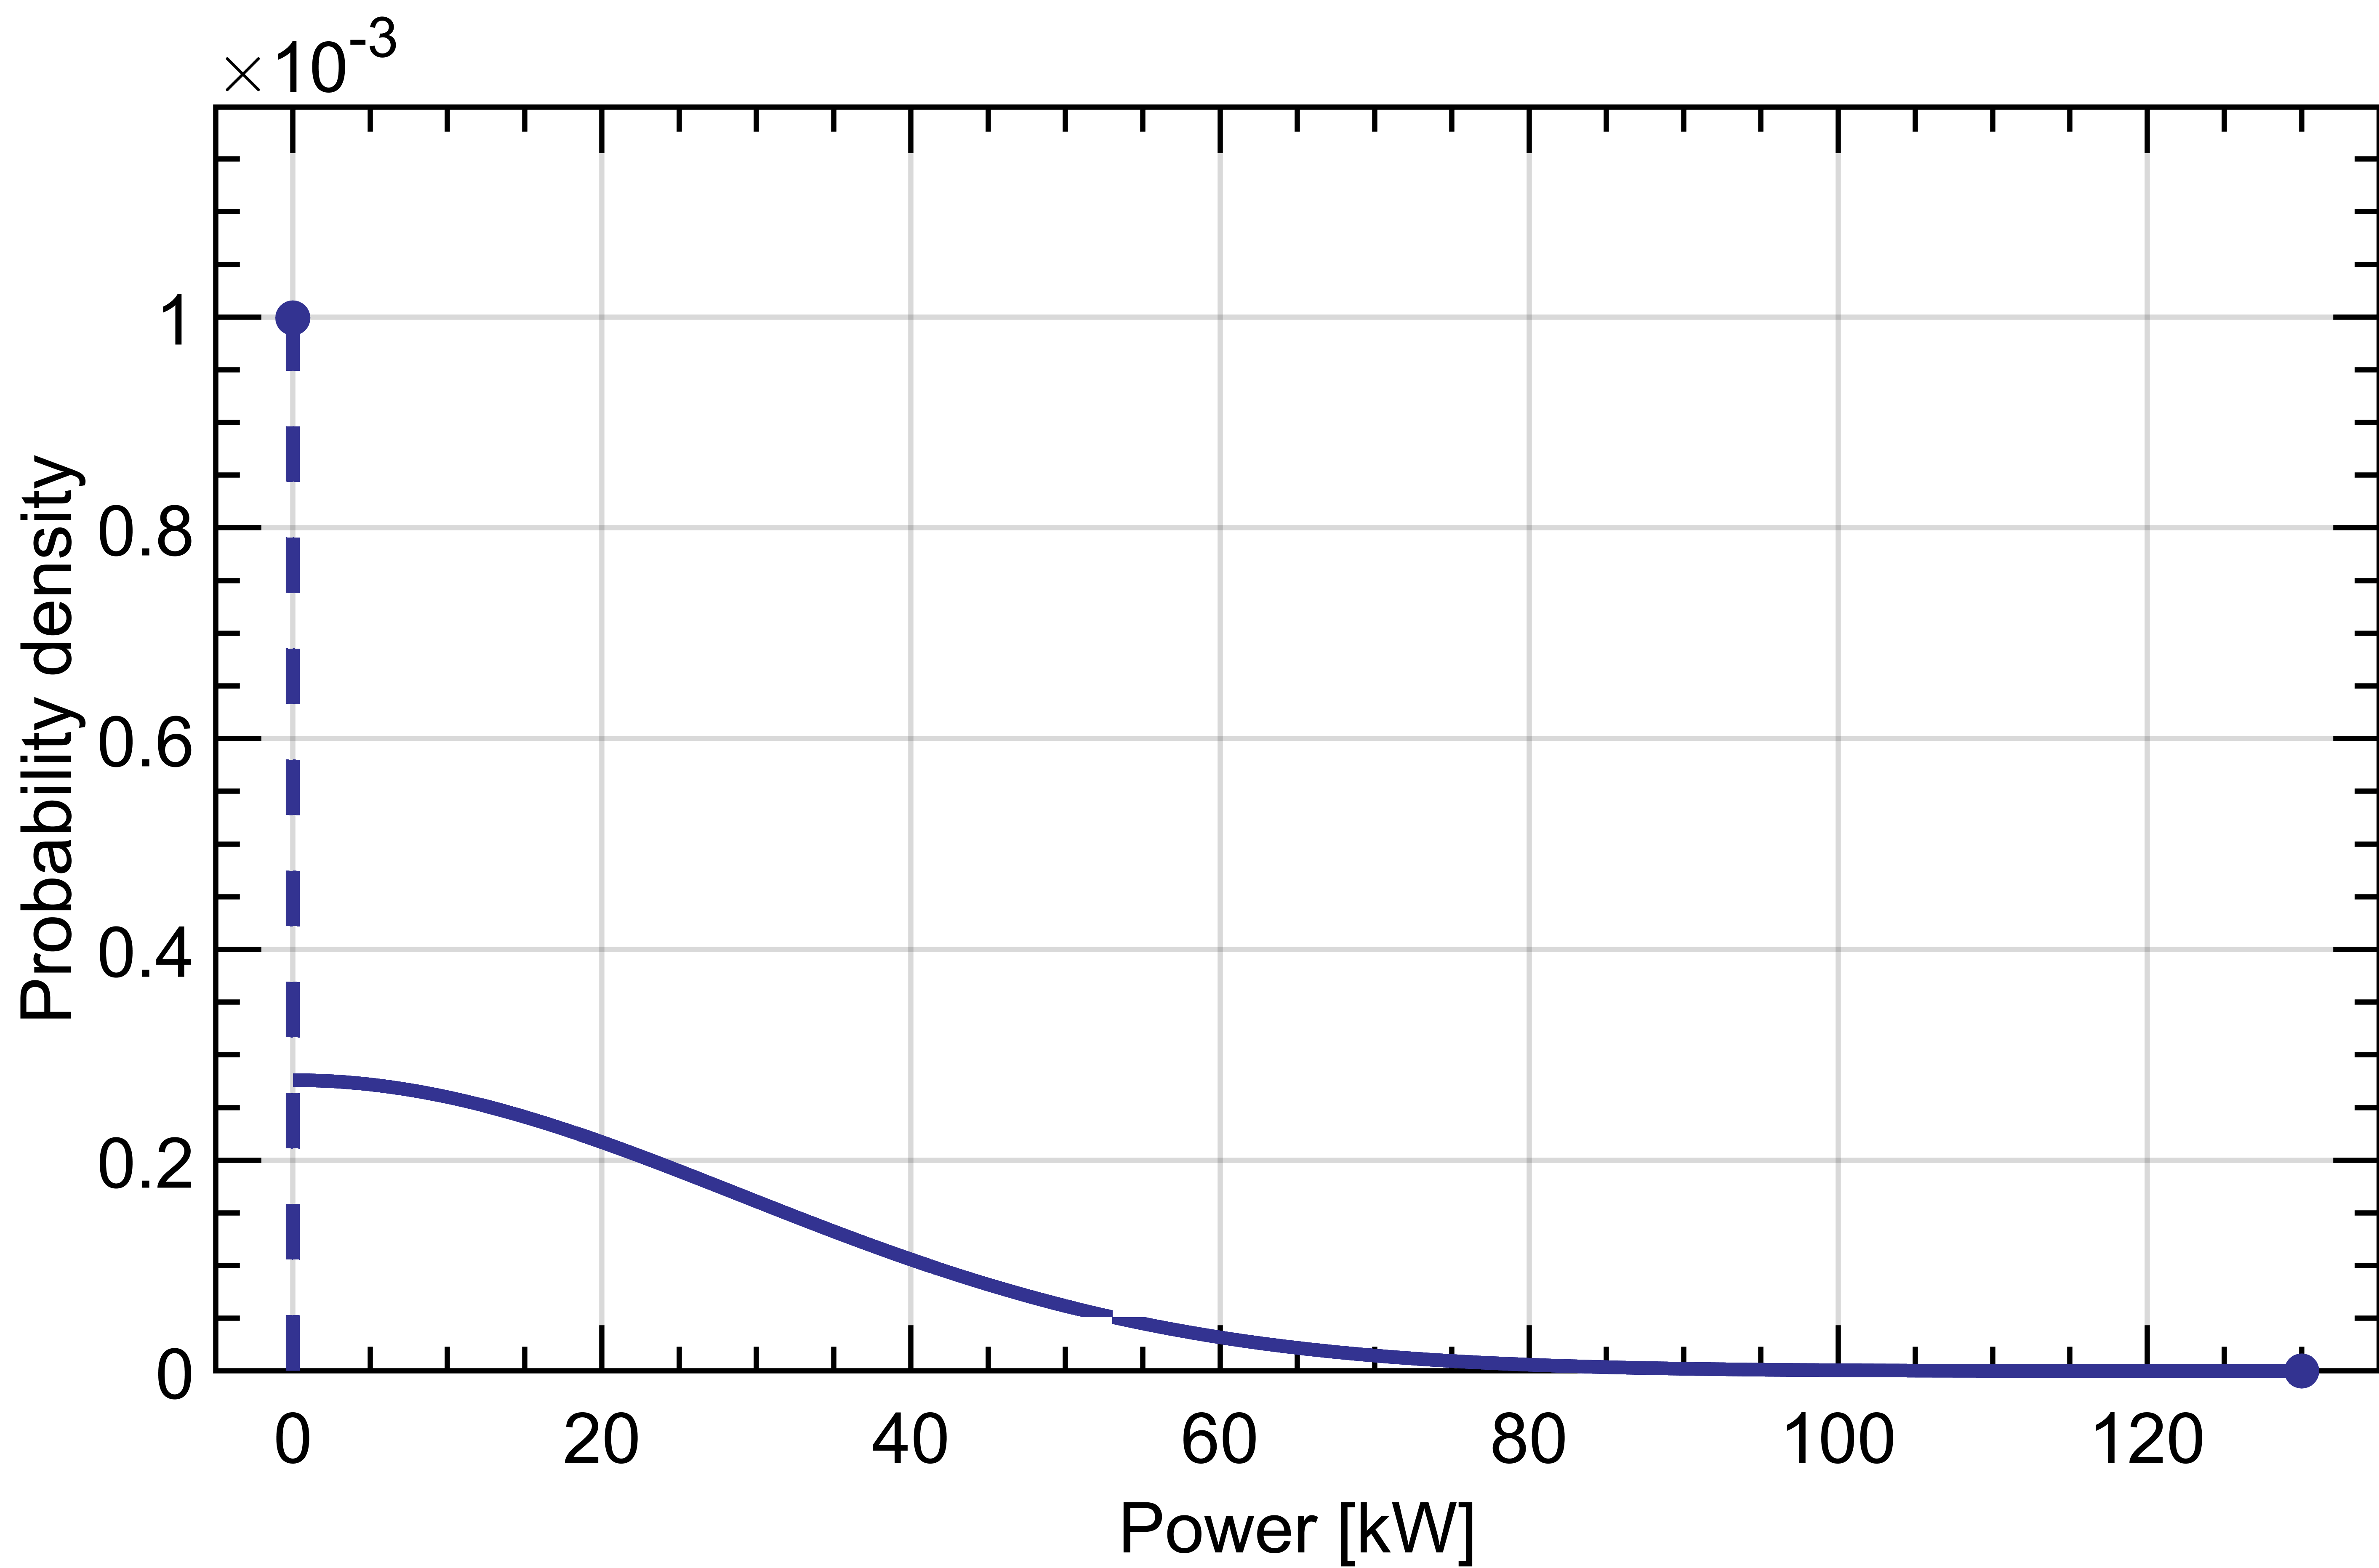
\includegraphics[width=0.5\textwidth]{02-figures/esempioFigura.png}
\caption{Esempio figura.}
\label{fig:Prova}
\end{figure}

Usare figure in .jpg o .png aumenta le dimensioni del file e ne riduce la qualità di stampa. Una soluzione può essere l'utilizzo di immagini in .pdf se sono schemi costruiti in Powerpoint oppure in .eps se figure generate in Matlab.
La prima figura è posizionata in alto, questo poichè è stato utilizzato il comando "t!". Per una panoramica sulle opzioni relative al posizionamento di figure, tabelle e algoritmi consultare \url{https://it.overleaf.com/learn/latex/Positioning_of_Figures}.

\begin{figure}[h]
\centering
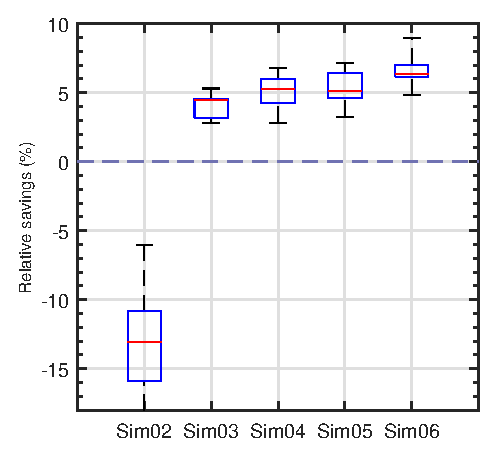
\includegraphics[width=0.5\textwidth]{02-figures/esempioFigura2.eps}
\caption{Esempio figura in formato eps.}
\label{fig:Prova2}
\end{figure}

\begin{figure}[H]
\centering
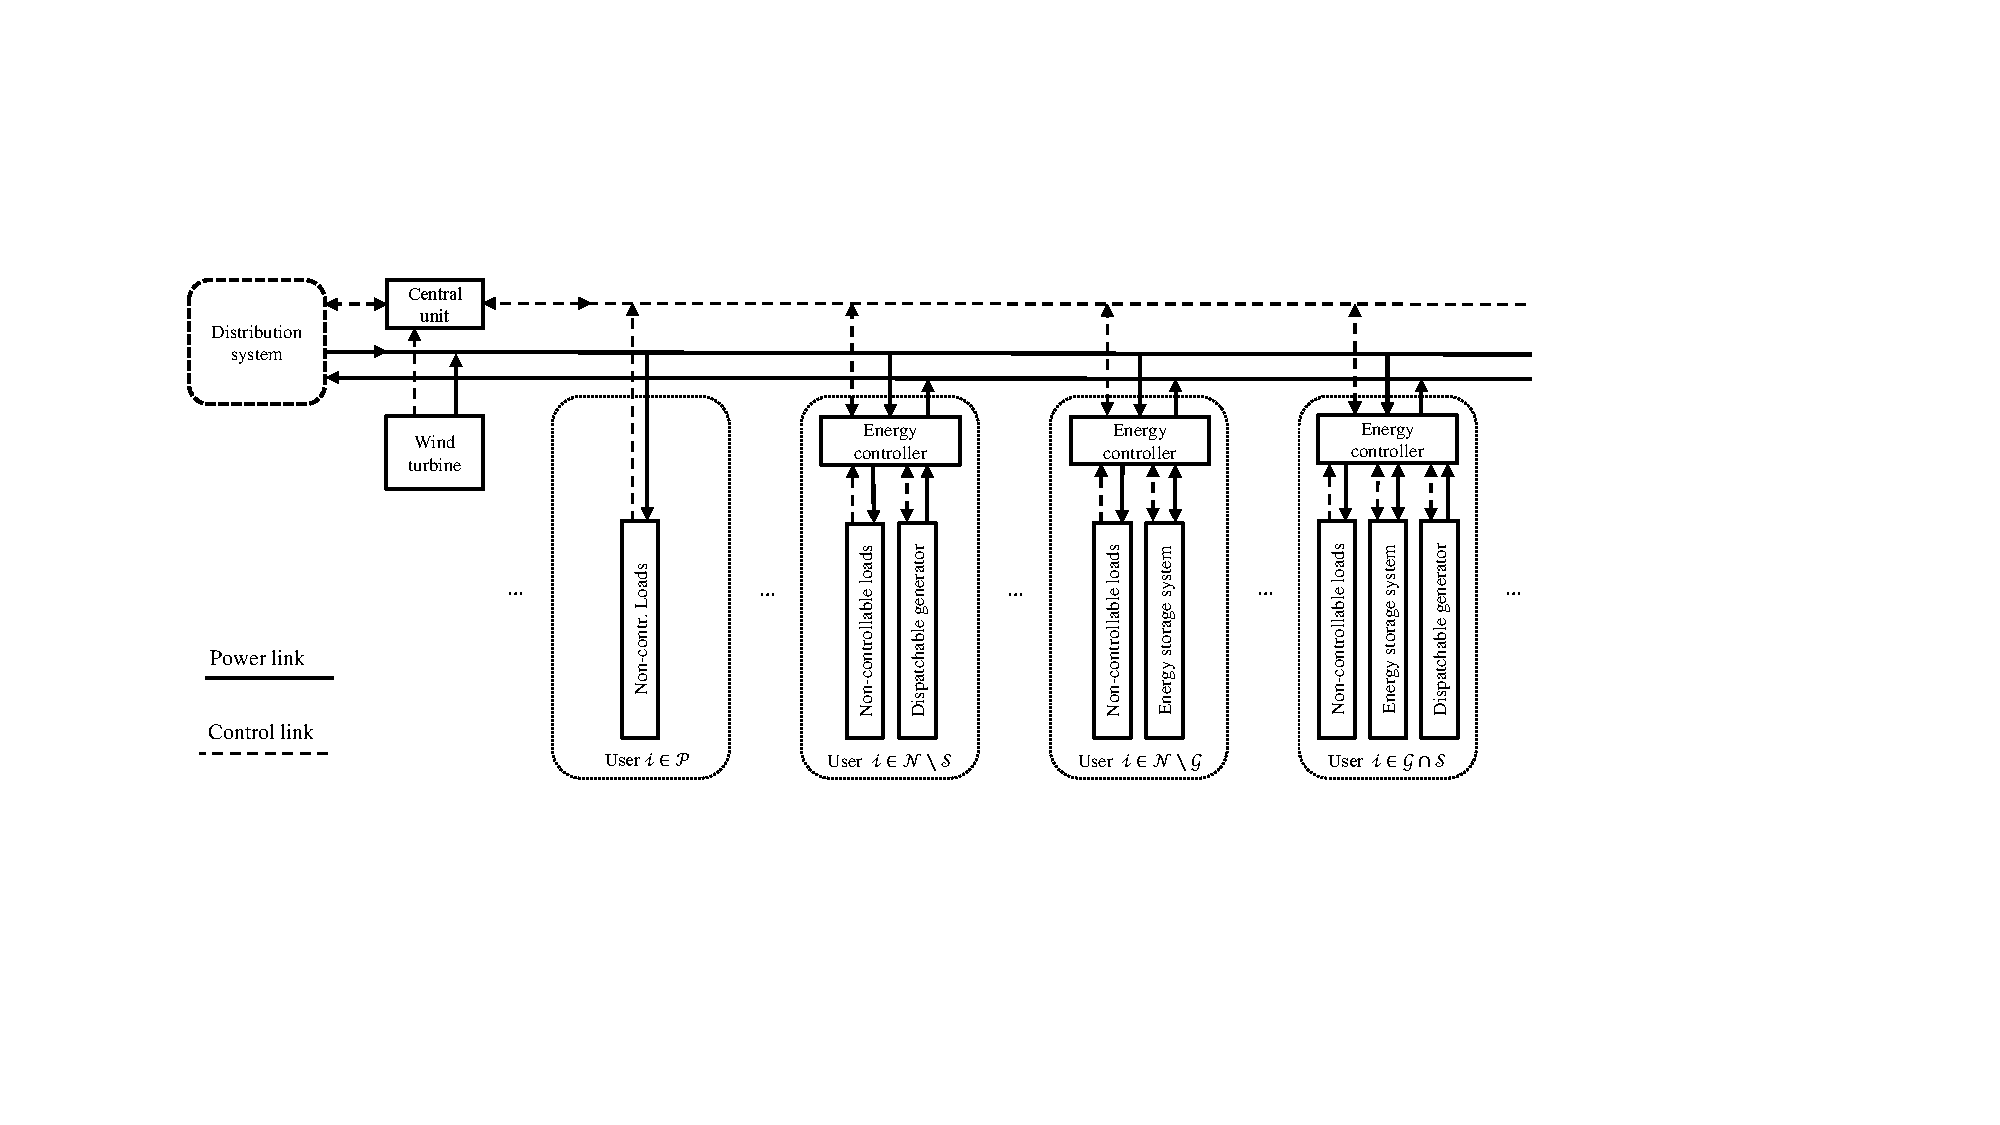
\includegraphics[width=0.8\textwidth]{02-figures/esempioFigura3.pdf}
\caption{Esempio figura in pdf.}
\label{fig:Prova3}
\end{figure}

\section{Descrizione del modello}
In questa sezione si presenta il modello matematico o il sistema oggetto dello studio: le ipotesi di partenza, le variabili e i parametri usati (con la stessa notazione che poi comparirà nelle equazioni), e le equazioni che lo descrivono. È il punto di riferimento a cui il lettore tornerà per capire cosa rappresentano le grandezze usate nelle sezioni successive, quindi conviene essere precisi ed espliciti fin da qui, anche a costo di essere un po' ridondanti.

\section{Simulazioni}
Questa sezione descrive le simulazioni numeriche condotte per validare o analizzare il modello presentato: lo scenario considerato, i valori dei parametri usati e il motivo per cui sono stati scelti, e infine i risultati ottenuti, tipicamente sotto forma di grafici o tabelle. Ogni caso analizzato può essere descritto in una propria sottosezione, come nell'esempio seguente.

\subsection{Caso 1}
Descrivere qui lo scenario specifico simulato (ad esempio un particolare valore di un parametro, o una condizione iniziale), i risultati numerici o grafici ottenuti (Fig./Tab. con riferimento, come visto in \S\ref{tab:tabellaEsempio}) e un breve commento che li interpreti: cosa si osserva, se è in linea con le aspettative teoriche, ed eventuali limiti della simulazione.

\section{Conclusione}
Le conclusioni riprendono lo scopo della tesina enunciato nel sommario e nell'introduzione, riassumono brevemente cosa è stato fatto e quali risultati sono stati ottenuti, e ne danno una valutazione critica: il modello si è comportato come atteso? Ci sono limiti evidenti nell'approccio seguito? Si può concludere con eventuali sviluppi futuri o domande aperte che il lavoro svolto ha fatto emergere.

%%%%%%%%%%%%%%%%%%%%%%%%%%%%%%%%%%%%%%%%%%%%%%%%%%%%%%%%%%%%%%%
%% FINE DEL DOCUMENTO
%%
%%
%%
%%%%%%%%%%%%%%%%%%%%%%%%%%%%%%%%%%%%%%%%%%%%%%%%%%%%%%%%%%%%%%%
% STAMPA DELLA BIBLIOGRAFIA (NON MODIFICARE
\printbibliography[heading=bibintoc,title={Riferimenti}]
%\printbibliography[heading=bibintoc,title={References}] % Per tesina in inglese decommentare

%%%%%%%%%%%%%%%%%%%%%%%%%%%%%%%%%%%%%%%%%%%%%%%%%%%%%%%%%%%%%%%
% Appendice
\appendix
% I codici vanno caricati direttamente su Overleaf, nella sottocartella
% del linguaggio (03-code/matlab oppure 03-code/python), e richiamati
% nel testo con "lstinputlisting".
\section{Codice Matlab}
\lstinputlisting{03-code/matlab/Codice1.m}

\section{Codice Python}
Per il codice Python si usa lo stile "pythonstyle" definito nel pacchetto del laboratorio:
\lstinputlisting[style=pythonstyle]{03-code/python/Codice1.py}
%%%%%%%%%%%%%%%%%%%%%%%%%%%%%%%%%%%%%%%%%%%%%%%%%%%%%%%%%%%%%%%
%%
%%
%%
%%%%%%%%%%%%%%%%%%%%%%%%%%%%%%%%%%%%%%%%%%%%%%%%%%%%%%%%%%%%%%%
\end{document}
% FINE